\section{Design} % (fold)
\label{sec:design}
The main goal of the \emph{Realms} system is to help in the creation of simple \emph{location-based applications} based on a configuration process and consists of the following three major components:
\begin{itemize}
	\item \emph{configuration manager} - empowers users with the possibility of augmenting a physical space with virtual properties and rules (we call it a \emph{realm})
	\item \emph{mobile client} - collects relevant context data and intermediates the interaction between the users and the system
	\item \emph{infrastructure} - holds the configured virtual spaces and guides the user-system interaction based on each user's context (location) information and posible virtual properties of the system (which can be applied in the user's context).
\end{itemize}
\\\\
There are two end user types which will use our system: the \emph{configuration managers}, which will create realms, and the \emph{?mobile client users?} which will interact with the realms using the provided mobile client. Actually, the mobile client users are end-users both to us and the configuration managers: they are our end-users because they will be using the mobile client, that we provide, to connect to one of the realms, provided by configuration managers.
\\\\
Indoors positioning needs a lot more infrastructure than the one provided by GPS satellites which makes indoor locations hard to deal with. Hence, we consider indoors spaces to be out of scope for our system and the realms which a configuration manager will be able to create can be based only on outdoors spaces. Therefore, we are excluding the possibility of indoors usage of the application and the mobile clients are meant to work only outdoors.
\\\\
The main advantage over similar system is that we empower users to create a ready-to-be-used context-aware application without writing one line of code.\\
\\\\
The whole system is built around three main entities: \emph{location information}, \emph{virtual properties} and \emph{rules/decisions} to govern the data; hence, we are dealing with a distributed, data-driven system. Our design will follow the client-server design pattern based on a data-drive client-server interaction.
\\\\
\begin{figure}
	\centering
	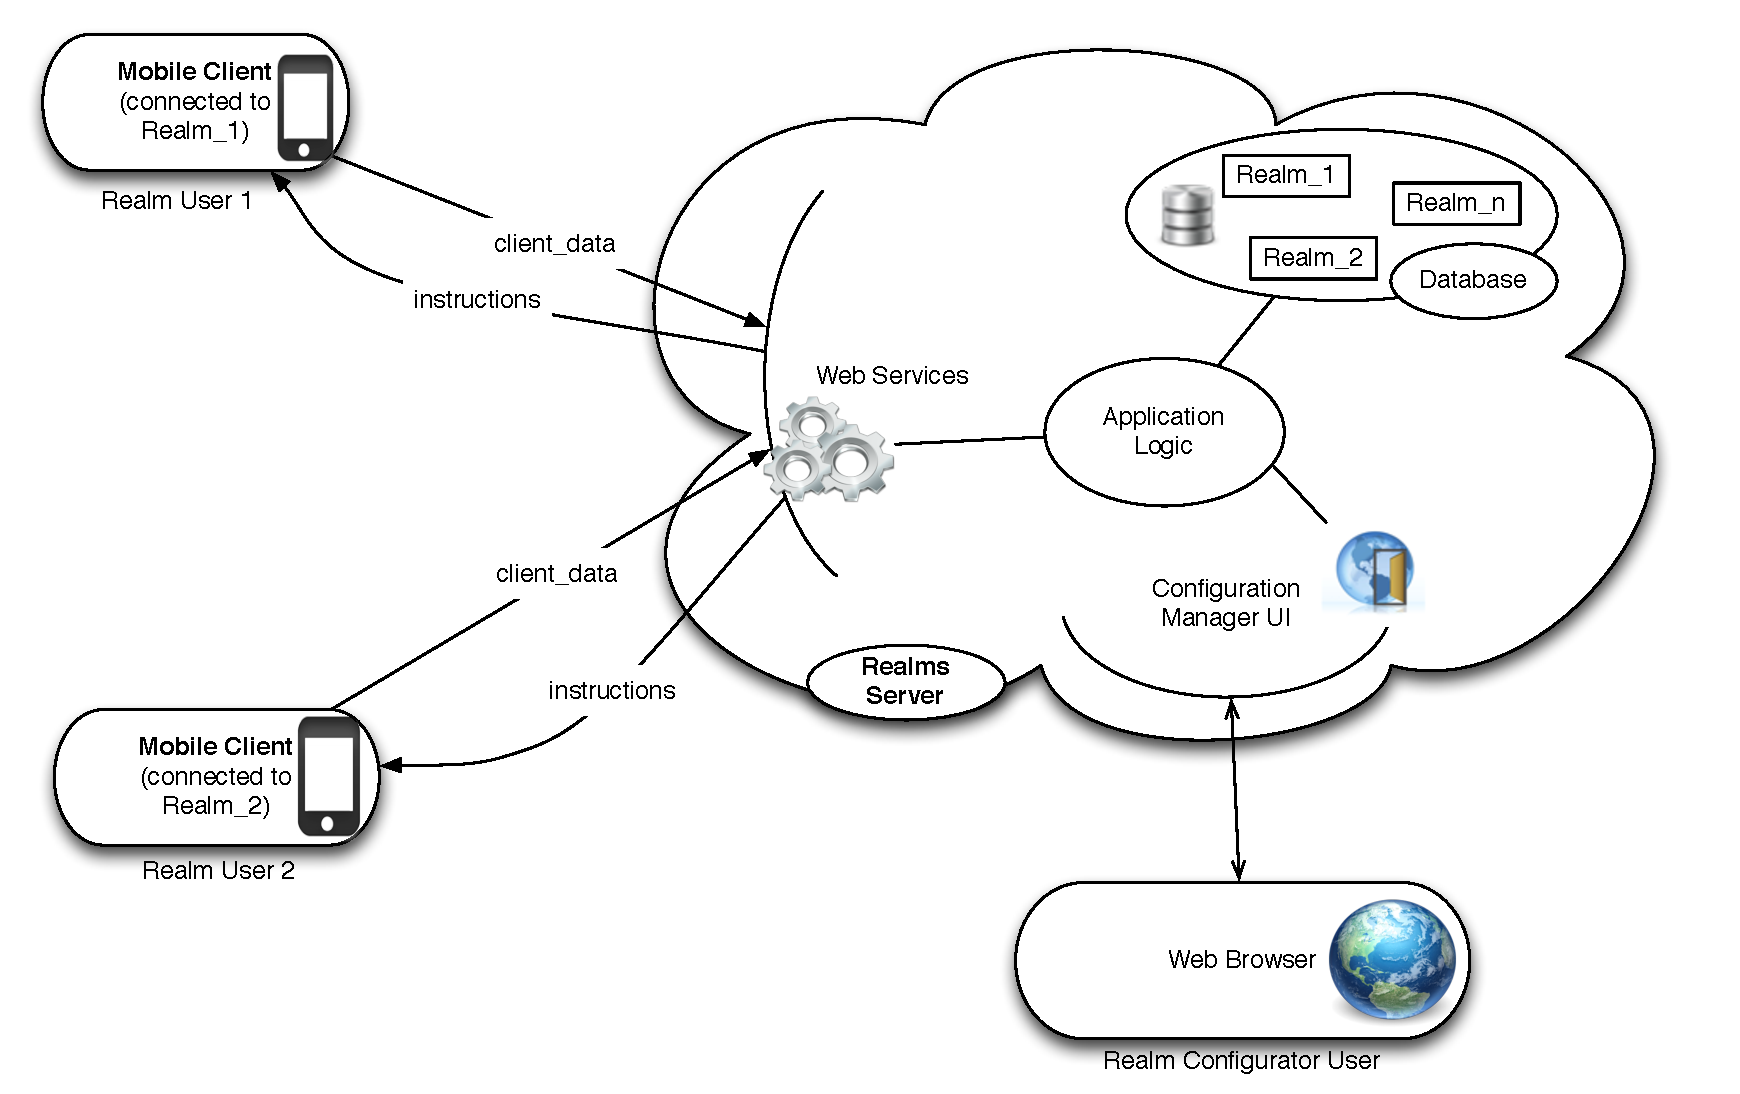
\includegraphics[width=0.9\linewidth]{fig/realms_high_lvl}
	\caption{High level system overview}
	\label{fig.design.high_lvl}
\end{figure}
Figure \ref{fig.design.high_lvl} depicts the major components and data structures of the system. On one hand we have the \emph{mobile clients} connected to the realms server, interacting with one of the realms and on the other hand we have the \emph{configured realms}, created by the \emph{configuration manager}, and the \emph{realms server} driving the interaction. The mobile clients communicate with the sever sending over the sensed data which, together with the virtual properties of the current realm, provides the server the necessary data to compute the next instructions for the client. Figure \ref{fig.design.comm_protocol} further details the interaction between the mobile client and the server.
\\\\
\begin{figure}[H]
	\centering
	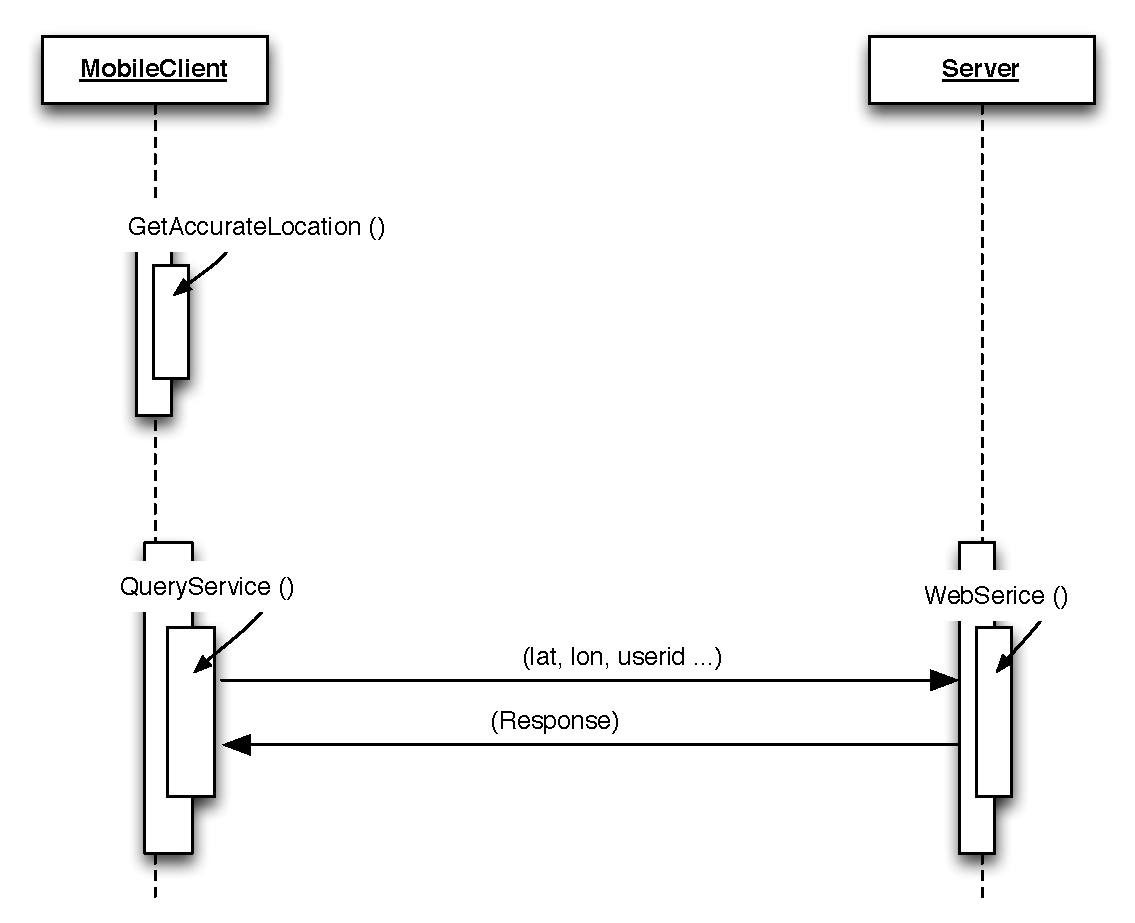
\includegraphics[width=0.9\linewidth]{fig/abstract_communication_protocol}
	\caption{Abstract Communication Protocol}
	\label{fig.design.comm_protocol}
\end{figure}
After the client is started up it tries to communicate with the realms server sending over the authentication credentials and a \emph{realm} to connect to. If the authentication is successful, the server either creates a new session or resumes and existing one; the way we manage the user sessions is an important characteristic of the system -- we are supporting long-running communication session between mobile phones and a server. The data connectivity of a mobile phones is still highly volatile so we have to consider as a fact that client-server communication can be broken at any time. We try to overcome this problem by storing each user session ID (and any relevant data), for each separate realm, in a persistent storage. When the mobile client starts to communicate with the server on a specific realm, the realms server will determine whether a new sessions has to be created or an existing one can be resume.
\\\\
Once the client got a connection to the server a series of \emph{report status data} - \emph{get instructions} will follow. The client gathers \emph{location data} and communicates it to the server which, using the information of the realm the client is connected to, computes the \emph{instructions} to be back to the client. The communication stops in one of the following situations: an exception occurs during the communication session, the client exists or the interaction flow got to an end.
\\\\
Finally, as we will shortly describe the concrete architecture we base our infrastructure and communication upon. \emph{REST} is an architecture style for distributed hypermedia systems. A \emph{web service} is an API which is accessed through the HyperText Transfer Protocol (HTTP) and executed on a remote system, hosting the requested service. A \emph{RESTful web service} is a web service implemented using HTTP and the principles of REST. The RESTful web service is defined by a collection of resource, each of which is defined by three main characteristics:
\begin{itemize}
  \item the base URI identifying the web service
  \item the MIME\footnote{Multipurpose Internet Mail Extensions} type of the
  data supported by the web service (JSON, XML, etc.)
  \item the web service's interface defined against the HTTP supported methods
  like POST, GET, PUT, DELETE etc.
\end{itemize}
\\\\
The REST architectural style imposes a client-server architecture, which fits well our system's architecture, which is also based on a client-server approach.

\subsection{Configuration Manager} % (fold)
\label{sub:configuration_manager}
The role of the configuration manager is to present a user with an interface where location-based interactions can be defined as they should appear in the mobile app. There are two aspects when creating configuring a realm -- on one hand there is the interface where concrete locations are augmented with virtual properties, and on the other hand there is the flow describing the interaction path between a client and the server.
\\\\
The most intuitive interface to augment physical location is a virtual map. This can be easily be browsed by concrete physical locations (latitude and longitude), city name, place name, address etc. These features make it easy for the user to rapidly find the desired location they want to augment. The configuration process will result in a list of (location, information) pairs where location is always \emph{(latitude, longitude)} and \emph{information} is a simple JSON string. The semantics of the information will be interpreted in the interaction flow. In this initial implementation of the system, the information will only be a list of options which will be transmitted to the client and their choice will be taken into consideration during the interaction flow.
\\\\
\begin{figure}[H]
	\centering
	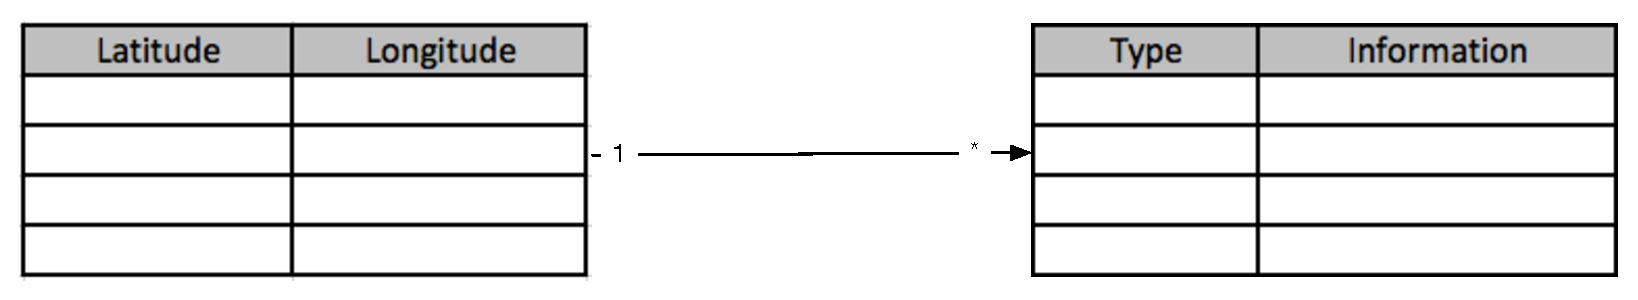
\includegraphics[width=0.9\linewidth]{fig/virtual_properties}
	\caption{Augmented Location Data}
	\label{fig.design.virtual_properties}
\end{figure}
As depicted in Figure \ref{fig.design.virtual_properties} the data will be stored in a database where concrete locations are in relation with augmented information. As the semantics of the information can be identified through their \emph{type}, this approach allows to easily enrich the types of information supported by the system in the future.
\\\\
In order to enable the user to easily specify the interaction flow between the client and the server we will employ the \emph{workflow} mechanism as it is the main mechanism to  capture and develop human-to-machine interaction. A workflow which consists of a sequence of concatenated (connected) steps. Emphasis is on the flow paradigm, where each step follows the precedent without delay or gap and ends just before the subsequent step may begin. Figure \ref{fig.design.workflow} illustrates the concept of the workflow applied to our system. Each workflow has a \emph{Start} and an \emph{End} and a number of \emph{intermediate steps}. Each step of the workflow has as entry the user's current location, the optional choice of the user (based on the virtual data assigned to the user's location) and the virtual properties present at the user's location. Based in this information the step at hand will be able to decide which is the next step and when the transition will be made.
\\\\
\begin{figure}[H]
	\centering
	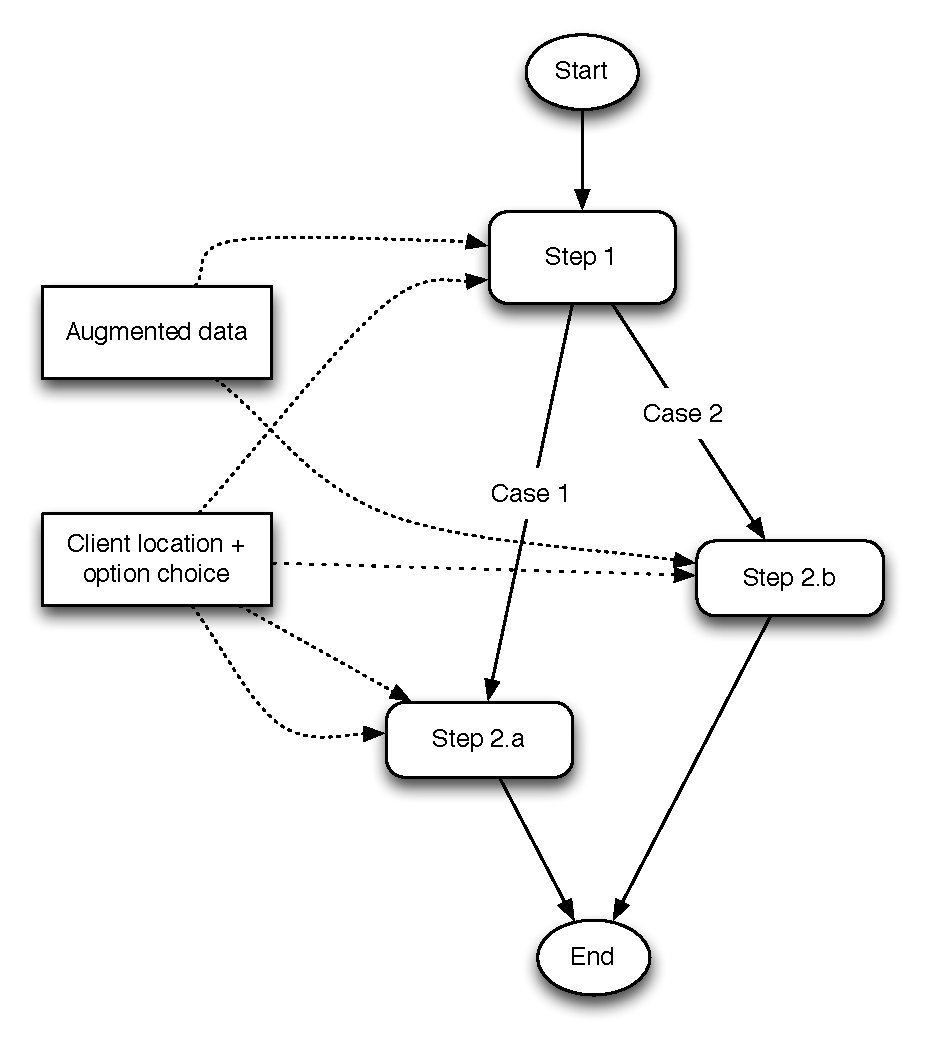
\includegraphics[width=0.9\linewidth]{fig/workflow}
	\caption{Worflow concept illustrated}
	\label{fig.design.workflow}
\end{figure}
The workflow builder is represented by a graphical tool where the user can create steps and connections inside the flow. For each step simple \emph{if-then-else} decision constructs will can be applied using the above mentioned variables (user location, virtual properties and optional user choice) and optional custom constants.
\\\\
\todo{insert schetch of UI here!}
% subsection configuration_manager (end)be available having 

\subsection{Realms Server} % (fold)
\label{sub:realms_infrastructure}
In this subsection we will describe our system infrastructure. The realms infrastructure is the backend of our system and handles connection from the mobile app and the configuration manager, and stores information such as location-based information and configurations.
% subsection realms_infrastructure (end)

\subsection{Realms Android App} % (fold)
\label{sub:realms_android_app}
In this subsection we describe our Android application. The app presents users with the ability to access realms and interact in them as described by their configuration.
% subsection realms_android_app (end)
% section design (end)